\chapter{绪论}

\section{引言}
子痫前期(preeclampsia, PE)又作先兆子痫,是孕妇妊娠期特有的一种多系统进展性疾病, 与妊娠期高血压(gestational hypertension)、子痫(eclampsia)、
慢性高血压并发子痫前期(chronic hypertension with superimposed preeclampsia)以及妊娠合并慢性高血压(chronic hypertension)统称妊娠期
高血压疾病(hypertension disorders of pregnancy, HDP)\cite{OAG9,HDASOM,2000s1}。
子痫前期临床表现的显著特点是原发性高血压与蛋白尿。
近年来,组织的对子痫前期的涵盖范围进行了进一步的拓展,在妊娠20周后出现新发(原发)高血压,在两次间隔$4h$或$4h$以上的血压测定中,收缩压≥$140mmHg$和(或)
舒张压≥$90mmHg$,且伴有下列任一项或多项\cite{OAG9,FIGO}:
\begin{itemize}
    \item 孕妇出现蛋白尿症状,尿蛋白≥$300mg/24h$,或尿蛋白/肌酸酐比值≥$30mg/mol$,或随机尿蛋白≥(+);
    \item 孕妇无尿蛋白但伴有以下任一器官或系统功能紊乱、受累受损:心、肺(肺水肿)、肝(血清转氨酶水平为正常值2倍以上)、肾(血肌酐水平大于$1.1mg/dl$
    或为正常值2倍以上)等重要器官,或血液系统(血小板<$100 \times 10^{9}/L$)等)、消化系统、神经系统的异常改变等;
    \item 胎盘-胎儿受到累及:胎盘胎儿生长受限、脐动脉多普勒分析检测异常、死胎等。 
\end{itemize}

妊娠期高血压疾病可引起严重的母胎并发症,是孕产妇和围产儿病死率升高的主要原因\cite{OAG9}。
据世界卫生组织统计,子痫前期在孕妇中发病率高达5\%-10\%,是除体内大出血外孕妇死亡的第二大危险因素\cite{LCT2006},每年可导致全球范围内约76 000名孕妇死亡,并进一步导致约500 000
名胎儿/婴儿的死亡\cite{DAM2015,LCT2006}(如\autoref{fig:dhd}所示)。为推广普及人们对危及母婴生命安全的子痫前期的认知,同时教育女性了解她们当前及长期的健康风险,
全球孕妇保健组织自2017年起将每年的5月22日确定为世界子痫日(world preeclampsia day)(如\autoref{fig:wpd}所示)。
\begin{figure}[htb]
    \centering
    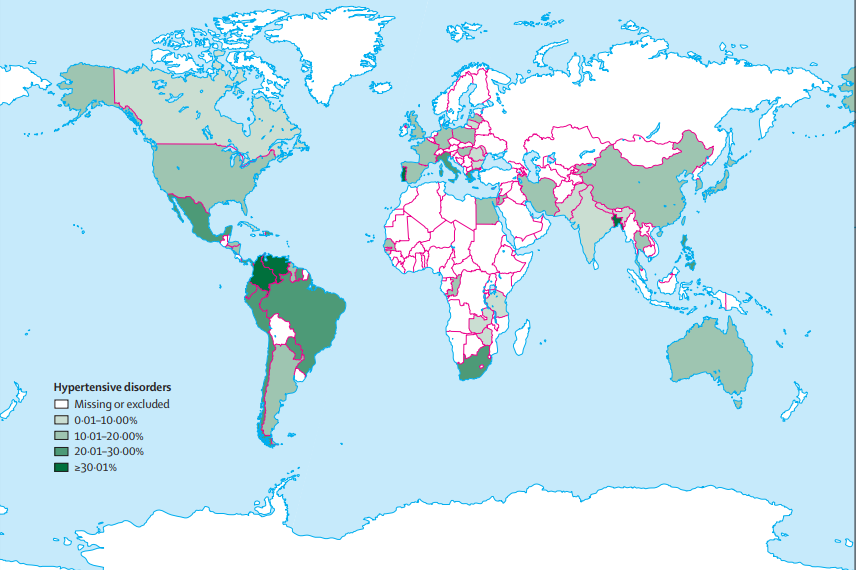
\includegraphics[width=.7\linewidth]{ch1/dhd}
    \caption{\label{fig:dhd}因妊娠期高血压疾病死亡孕妇的国家分布比例}
\end{figure}
\begin{figure}[htb]
    \centering
    
\includegraphics[width=.7\linewidth]{ch1/wpd}
    \caption{\label{fig:wpd}2021年世界子痫日主题:Preeclampsia: Beyond Pregnancy}
\end{figure}

就现阶段我国国情而言,由于人口基数大、人口出生率较高,导致每年妊娠孕妇数及新生儿数总量大。
同时,自全面开放二孩政策后,各地区高龄孕妇、二次妊娠孕妇比例明显提升。而临床研究已经证实,
高龄与二(三)次妊娠均属于可能导致子痫前期的风险因素,会增加孕妇子痫前期的患病可能。

因此,如何对子痫前期快速有效的医学诊断与干预成为新的难题,实现子痫前期的预测和及早诊断,
是对孕妇子痫前期的治疗及孕妇、围生儿的健康安全的保障,具有重大的临床应用价值。
\section{子痫前期的病理及危害}
\subsection{病因及发病机制}
截止目前,医学界对子痫前期的病因与发病机制尚未完全明确,相关研究还在继续进行之中。但得到公认的一点是,子痫前期病发具有异质性,多因素、多机制及多通路均对子痫前期的发病有所影响,不能仅以“一元论”的观点对待。
目前最为普遍接受的一种观点认为,子痫前期的发病与妊娠早期胎盘功能紊乱密切相关,其作用机制可以概括为两个阶段。
在第一阶段,孕妇子宫螺旋动脉重构受损、出现重铸障碍,导致胎盘缺血、缺氧,释放多种胎盘因子,该阶段无明显临床现象;在第二阶段,各种胎盘因子进入母体血液循环,促进系统性炎症反应的激活及血管内皮损伤引起子痫前期-子痫多样化的临床表现。有关病因和发病机
制的主要学说有以下几种:


螺旋动脉重构受损尤其被认为是导致先兆子痫的早期但不一定是原发性缺陷。19重构是一个多步骤过程20,其中第一个相关步骤应在植入前后开始。
这一阶段的紊乱可能增加先兆子痫的风险,并可能解释其在不明原因的低生育率或反复流产妇女中的较高发病率。21,22蜕膜相关血管变化也出现在子宫内膜(结合区)肌层,随后是滋养层细胞入侵并伴有相关的重塑。23滋养层细胞HLA-C、HLA-E
和HLA-G与子宫自然杀伤细胞或树突状细胞或两者的相互作用被认为对入侵的调节很重要,24-26以及HLA-C和杀伤细胞免疫球蛋白样受体亚型的某些组合易患子痫前期。

由于螺旋动脉和植入的囊胚壁中的腔隙之间出现连接通道,绒毛间流动似乎开始。28 早期滋养层堵塞可能保护胚胎免受高氧浓度的影响。研究人员 29 推测,这些栓塞的过早丢失可能导致过早流产,或者根据时间的不同,
会导致先兆子痫。通过滋养层的血管内迁移逐渐解决堵塞。绒毛间血流被认为是从外侧区域开始的,29 而滋养细胞的侵袭和相关的螺旋动脉出口的拔除始于中心并扩散到外围。绒毛间流动的外周开始应导致高局部氧化应激,
导致绒毛退化和绒毛膜叶的形成。因此,血管内堵塞的横向扩散不足可能导致广泛的绒毛膜退化和胎盘小,29 导致宫内生长受限、早发性先兆子痫或两者兼而有之。

在黄疸的胎盘氧曲线30上重叠的滋养层浸润和螺旋动脉重塑步骤表明,在胎盘氧急剧上升期间(10-12周),蜕膜和连接区子宫肌层中的蜕膜相关重塑发生,然而,在10周时,一些蜕膜动脉已经充满整个长度的血管内滋养层。
31在随后发展为子痫前期的妇女中,早在12周就可以检测到胎盘血流缺陷。32子宫肌层动脉段的深度侵犯发生在胎盘氧含量从15周开始急剧上升之后,因此可由血流增加触发。31因此,子痫前期子宫肌层螺旋动脉侵犯受损可能是由母体血流缺陷引起的,
而不是引起的。由于子宫肌层螺旋动脉比相应的蜕膜血管具有更明显的肌被和弹性,因此在此水平上的重塑失败会导致子宫胎盘动脉流量减少和胎盘灌注不规则。在某些情况下,此类缺氧或复氧事件会产生活性氧,33导致胎盘氧化应激和胎盘功能障碍,
伴有内质网应激和蛋白质合成受损。34我们认为,第一种(胎盘)原因不明子痫前期的阶段35可能包括对滋养层细胞的过度或非典型母体免疫反应,36以及蜕膜化受损或适当子宫预处理失败。37因此,子痫前期是两种基因不同的生物体之间相互作用失败的疾病。
因此,黑格的母胎冲突假说可能是相关的。38

与正常妊娠相比,系统性母体疾病的第二阶段(图)与过度的内皮激活和广泛的高炎症状态有关。 39 胎盘缺氧或再灌注的发作导致氧化应激,随后合胞体结构的凋亡和坏死破坏,40 和各种成分从绒毛间隙释放到母体循环中,刺激炎症细胞因子的产生。
 41 循环生物活性滋养层碎片包括合体滋养层膜微粒 41 和过量的合体滋养层衍生的抗血管生成因子,如可溶性内皮糖蛋白和血管内皮生长的可溶性形式因子 (VEGF) 受体 (sFlt-1)。18 最近在葡萄胎妊娠中也显示了滋养层细胞产生的抗血管生成因子增加,
 这是一种已知使女性易患先兆子痫的疾病。42,43 -eclampsia44 resu内皮功能障碍和相关血管反应性增加,在有症状的临床疾病发作之前。45 内皮完整性的丧失有助于钠容量稳态的紊乱和许多心血管变化(例如,心输出量和血管内容量增加)的逆转,伴随着正常妊娠。
 因此,先兆子痫是一种低输出、高抵抗的状态,具有矛盾的醛固酮和肾素活性降低。 46


 对于先兆子痫的几种表型,包括溶血、肝酶升高和低血小板计数 (HELLP) 综合征,1 期和 2 期之间的联系机制可能不同,47 有时因人而异。先兆子痫是早发(通常并发宫内生长受限)还是晚发取决于第 1 阶段的胎盘是否因血管生成失衡而变得表型变小。 
 48 胎盘不良不应被视为导致子痫前期的原因先兆子痫,因为并非所有此类妊娠的结局都不佳,而是作为一个强大的诱发因素。 39 如果胎盘大小适合胎龄,诱发心血管和代谢综合征样疾病也可能引发胎盘和全身炎症和氧化应激的级联反应,导致迟发性先兆子痫(也称为母体先兆子痫)。
  49 与早发性先兆子痫相比,迟发性先兆子痫中绒毛形态正常的发现证实了这一观点,50 尽管胎盘床似乎不存在此类数据。

  虽然母体遗传和体质因素与环境因素之间的相互作用促成了第二阶段,但现在认为这些因素对疾病的第一阶段有影响。 49 降低母体血液和 I 期和 II 期生物转化活性。蜕膜和胎盘组织可能导致先兆子痫风险增加。 51 吸烟对先兆子痫的保护作用 52 可能是由于一氧化碳对滋
  养细胞侵袭和螺旋动脉重塑的有益作用,增加了第 1 阶段胎盘血流量,减少了第 1 阶段胎盘血流量。 2 炎症反应。53 sFlt-1 的胎盘释放减少可能与这种保护作用有关。 54





1,子宫螺施小动脉重铸不足 正常妊娠时,细
高危因素
ne胞滋养层细胞分化为绒毛滋养细胞和绒毛外滋养  第一阶段
t1细胞(extravillous trophoblast,EVT),EVT包括间质第三阶1般氧化应激及胎盘浅猪床-「无临床征象
.绒毛外滋养细胞(interstitial extravillous trophoblast.
费症反应
1出现临床征乘
EVT)和血管内绒毛外滋养层细胞(endovascular ex-
travillous trophoblast,enEVT),iEVT负责浸润子宫1母体全身炎症反应
内膜基质直至子宫肌层的内1/3处,enEVT则进入
子宫螺旋小动脉管腔并逐渐替代血管壁平滑肌细
全身小动脉痉率1胞、内皮细胞,使动脉由高阻力低容量血管转变为
子梅前期-子痛
低阻力高容量血管以提高胎盘的血流量、确保母胎 图8-4 子痢前期发病机制“两阶段学说”示意图之间物质交换正常进行和胎儿发育。但子痫前期绒毛外滋养细胞泻
和子宫螺旋动脉重铸极其不足,仅蜕膜层血管重铸,子宫螺旋动脉1已完成等级加速,活跃天数1阻力增大,胎盘灌注减少,从而引发子痫前期的一系列症状。但造成子宫螺旋小动脉重铸 足的机制尚待研究。
品
2,炎症免疫过度激活 子痫前期患者无论是母胎界面局部还是全身均存在炎症保中激活现象。现有证据显示,母胎界面局部处于主导地位的天然免疫系统在子痫前期发病中起重要作用,Toll样受体家族、蜕膜自然杀伤细胞(dNK)、巨噬细胞等的数量、表型和功能异常均可影响子宫螺旋小动脉重铸,造成胎盘浅着床。特异性免疫研究集中在T细胞,正常妊娠时母体Th1/Th2免疫状态向Th2漂移,但子痫前期患者蜕膜局部T淋巴细胞向Thl型漂移。近年发现,CD4"CD25"调节性T细胞(regulatory T cell,Treg细胞)参与Thl/Th2免疫状态的调控。当Treg细胞显著减少时,促进Thl占优势,使母体对胚胎免疫耐受降低,引发子痫前期。
3,血管内皮细胞受损 血管内皮细胞损伤是子痫前期的基本病理变化之一,它使扩血管物质如一氧化氮(NO)、前列环素,合成减少,而缩血管物质如内皮素(ET)、血栓索A,等合成增加,从而促进血管痉挛。此外血管内皮损伤还可激活血小板及凝血因子,加重子痫前期的高凝状态。引起子痛前期血管内皮损伤的因素很多,如炎性介质:肿瘤坏死因子、白细胞介素-6、极低密度脂蛋白等,还有氧化应激反应。
4,遗传因素子痫前期具有家族倾向性,提示遗传因素与该病发生有关,但遗传方式尚不明确。由于子痫前期的异质性,尤其是遗传和环境因素的交互作用产生了复杂的表型。在子痫前期遗传易感性研究中,尽管目前已定位了十几个子痛前期染色体易感区域,但在该区域内进一步寻找易感基因仍面临很大的挑战。
现 食对题合
5,营养缺乏已发现多种营养因素如低白蛋白血症、钙、镁、锌、硒等缺乏与子痫前期发生发展可能有关,但是这些证据需要更多的临床研究进一步证实。

【病理生理变化及对母儿影响】
-基本病理生理变化是全身小血管痉挛和血管内皮损伤。全身各脏器各系统灌注减少,对母儿造成危害,甚至导致母儿死亡。由于该病表现为多脏器和系统损害,故有学者提出子痫前期-子痫综合征(preeclampsia-eclampsia syndrome)的概念。
1,脑 脑血管痉挛,通透性增加,导致脑水肿、充血、局部缺血、血栓形成及出血等。CT检查脑皮质呈现低密度区,并有相应的局部缺血和点状出血,提示脑梗死,并与昏迷及视力下降、失明相关。大范围脑水肿主要表现为感觉迟钝和思维混乱,个别患者可出现昏迷,甚至脑疝。子病前期脑血管阻1力和脑灌注压均增加,高灌注压可致明显头痛而子痫的发生与脑血管自身调节功能丧失相关。
2肾脏肾小球扩张,内皮细胞肿胀,纤维素沉积于内皮细胞。血浆蛋白自肾小球漏出形成蛋 m
尚未明确。

(一)下列因素易发生妊高征:

1.年轻初孕妇及高龄初产妇;

2.家族中有高血压或肾炎、糖尿病病史者;

3.体形矮胖;

4.多胎妊娠、羊水过多、葡萄胎患者;

5.经济条件差,营养不良,重度贫血者;

6.对妊娠恐惧,精神过分紧张或受刺激者;

7.寒冷季节、气压升高时发病增多。

(二)主要病因学说

1.子宫胎盘缺血学说:1918年Young首先提出子宫一胎盘缺血学说,认为临床上本病易发生于腹壁较紧的初产妇。多胎妊娠、羊水过多等,由于子宫张力增高,影响子宫胎盘间血液供应,或者全身血液循环不通适应妊娠子宫一胎盘的需要,如严重贫血、慢性高血压、肾炎等,导致子宫一胎盘缺血缺氧而发病。
此学说解释了临床现象,但没有阐明疾病的本质。

2.免疫学说:认为胎儿胎盘是具有半抗原性移植体,妊高征实质上是胎儿胎盘对母体诱导出的较强的免疫应答反应。精子内有组织相容性抗原(HLA)存在,如胎儿胎盘遗传得到HLA者,HLA处于免疫惰性状态,故能支持母亲免疫系统接受胎儿胎盘异体移植物,
反之,则可引起母体抗原抗体反应。临床上妊高征患者HLA抗体的检出率明显高于正常孕妇,妊高征患者蜕膜及胎盘血管动脉粥样硬化病变与移植器官时的血管病变相似;妊高征患者体液免疫与细胞免疫功能异常等,都支持免疫学说。

3.弥漫性血管内凝血(DIC)学说:妊娠期多数凝血因子增加,凝血功能增加,纤溶活性抑制,血液处于高凝状态。妊高征患者上述变化更显著,抗凝血酶(ATⅢ)减少,血容量减少,血液浓缩,加之血管痉挛,内皮损伤,胶原暴露,易出现血栓。缺血缺氧之胎盘变性坏死,释放促凝物质进入母体血循环,激发血管内凝血。妊高征患者血中纤维蛋白降解产物(FDP)增高,血小板减少,凝血功能检查异常,甚至有出血倾向,肾小球纤维蛋白沉积,胎盘梗死等均支持DIC学说。但妊高征与DIC的因果关系尚未肯定。

4.其他:近几年来,还有前列腺素合成失调,即具有血管收缩作用的血栓素(TXA2)增高,而具有扩张血管作用的前列环素(PGI2)相对不足而导致血管痉挛、血压升高。母体对血管紧张素Ⅱ的反应过度增强等新学说。有待深入研究。
\subsection{危害}

\section{子痫前期的研究现状}
现代医学对子痫前期的认知经历了漫长的探索\cite{BJOG2016}。
\subsection{发展史}
\subsection{风险因子}
\subsection{血压}
\subsection{生化指标}
生化指标(biomarker)
123

\begin{figure}[htbp]
    \centering
    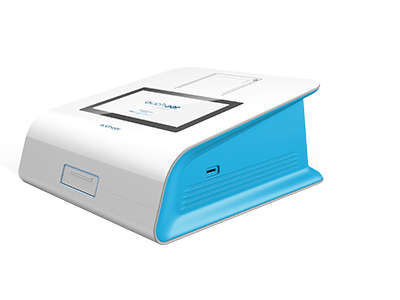
\includegraphics[width=.3\linewidth]{ch1/aocheng_kit}
    \caption{\label{fig:aocheng_kit}胎盘生长因子检测试剂盒}
\end{figure}
123

\subsubsection{1}

\subsection{人工智能技术}
今年来,由于计算机领域人工智能技术的高速发展,以及现代化设备的普遍使用,
相关研究者也开始尝试在子痫前期的识别、判断乃至预测等研究内容上引入人工智能技术。

\subsection{存在的不足与分析}
综合上述分析,对子痫前期的早期识别与检测可从按以下思路开展深入探索与研究。



\section{脉搏波在子痫前期领域研究现状}



\section{脉搏波时域特征研究现状}

\section{用脉搏波检测子痫的优势}
\section{研究目标与内容}

\subsection{研究目标}
综合应用各种方法,提取研发新型光电容积脉搏波形态学特征参数,构建一般通用的光电容积脉搏波的描述特征集合。在此基础上,通过特征筛选、压缩等算法提取出对子痫前期有一定甄别能力的特征集,
使用机器学习算法构建出子痫前期筛选识别模型,并对最终模型的性能表现进行验证评估。
\subsection{研究内容}
全文研究内容可分为数据源获取、信号预处理、特征参数提取与分析、子痫前期甄别模型训练构建及模型评估具体包括5个部分,如所示。每部分具体研究内容包括:
\begin{enumerate}
    \item 数据源获取。介绍本研究所采用的数据来源(临床现场采集),包括采集设备、采集流程及规范。  
    \item 信号预处理。对从硬件设备获取的PPG信号分析其信号成分特点,完成滤波去噪、去基线漂移、特征点检测及标准化等准备工作。
    \item 特征参数提取与分析。从脉搏波形态学等方面构建特征参数。
    \item 子痫前期甄别模型训练构建及评估。通过机器学习中的等方法构建子痫前期甄别模型,并验证模型准确性。
    \item 模型评估。
\end{enumerate}

\textbf{各章节的具体内容安排如下:}

第一章是绪论。介绍子痫前期的定义及危害,梳理了目前临床已应用的检测方法及指标,分析各项方法的缺陷与不足。最后确定提出了本文的研究目标与内容。

第二章是子痫前期及光电容积脉搏波的生理学基础。阐述了

第三章是光电容积脉搏波的特征点检测算法。

第四章是光电容积脉搏波的特征集构建。

第五章是基于光电容积脉搏波特征的子痫前期检测识别模型。通过等几种方法优化特征参数集并构建了子痫前期的甄别模型,通过等方面评估了各项模型的整体性能表现。

第六章是低耦合高拓展的软件综合分析系统的设计与实现。阐述了本研究包括数据源导入管理、预处理算法管理、特征拓展管理、标准数据管理、模型训练生成管理等方面在内的整体分析系统的软件设计思路,
介绍了为提高本研究各部分内的内聚性、降低各研究内容之间的耦合性、提高系统整体可拓展性及实用性、提高系统真正落地临床的可能性所做出的各项规划及实现。

第七章是总结与展望。对本论文的全部研究工作进行系统性总结,阐述本论文的创新工作点,并对下一阶段的研究工作内容进行了规划与展望。

\chapter{生理学基础}
\section{引言}
由于本研究开展所使用的脉搏波数据均为通过光电容积描述标记的方法无创所得,因此在本章最后进一步阐述了微循环容积脉搏波血流模型及光电容积脉搏波采集原理。
\section{子痫前期的生理学基础}
妊高征基本的病理生理变化是全身小动脉痉挛和水钠潴留。

(一)全身小动脉痉挛 可能由于升压系统和降压系统平衡失调,血管壁对某些升压物质(如血管紧张素Ⅱ)的反应性增强,从而使全身小动脉,特别是直径200um以下的小动脉发生痉挛,导致各器官供血不足,外周阻力增高,产生高血压等一系列症状体征。

子宫血管痉挛,胎盘供血不足,绒毛退行性变、出血、坏死、梗塞等,导致胎盘提高老化,功能不全。病变进行缓慢时,可致胎儿宫内生长发育迟缓(IUGR),病变急剧时,可致胎死宫内,严重时胎盘后小血管破裂,导致胎盘早剥。

脑部血管痉挛,脑组织缺氧、水肿、严重时出血,出现头昏、头痛、恶心、呕吐,重者抽搐、昏迷,脑疝形成而致死亡。

心脏血管痉挛,心肌缺血、间质水肿、点状出血及坏死,加之血液粘稠度增加,外周阻力增加,心脏负担加重,可导致左心衰竭,继而发生肺水肿。

肾脏血管痉挛,肾血流量减少,组织缺氧,血管壁通透性增加,血浆从肾小球漏出,出现蛋白尿及管型。肾小球毛细血管痉挛,肾小球内皮细胞肿胀,发生血管内凝血,纤维蛋白沉着,肾小球滤过率减少,出现尿少,严重者出现肾功衰竭。

肝脏由于缺血,肝细胞线粒体内所含的谷丙转氨酶释放,可致血清谷丙转氨酶升高,出现黄疸表明病情严重。肝脏主要病变为门静脉周围有局限性出血,继而纤维素性血栓形成,严重者肝实质缺血坏死、肝包膜下出血。

眼底小动脉痉挛、缺血、水肿,严重时渗出、出血,甚至视网膜剥离,出现眼花、视物模糊,甚至失明。

(二)水钠潴留 可能由于肾小球滤过率减少,肾小管对钠的重吸收增加,钠离子潴留细胞外而引起水肿。肾上腺皮质激素、抗利尿激素分泌增加,也可能是水潴留的另一个原因。由于水钠潴留,组织水肿,体重异常增加。
\section{光电容积脉搏波概述}
\subsection{脉搏波产生原理}
\subsection{生理参数与非生理参数建立的心血管模型}
按照信号与系统的观点,若干相互作用、相互联系的事物按一定规律组成具有特定功能的整体均可称为系统,而信号则是反映信息的各种物理量,是系统直接进行加工、变换以实现通信的对象。而在脉搏波的工程研究领域,
人体的动脉管系亦可视为一个力学系统,心脏搏动作为该系统输入,而人体各处采集获得的脉搏波即为该系统输出(响应)。可由该系统的输入输出关系分析推断其结构特性参数,进一步研究脉搏波其他特性。\cite{PPGYY}

为尽可能精确描述心血管系统、探求心血管系统的生理特性,多年来学者们提出并建立了各种不同的数学模型进行拟合。而这些心血管模型大体上可依据建立时是否使用多个变量去拟合还原血液在血管中的可能涉及的血压、
血流弹性、阻力等生理变量分为生理参数模型与非生理参数模型两大类。\cite{PPGYY}生理参数模型关注心血管系统中的所有细节,模型中的各个参数变量均有较好的解释,也能与实际生理病理现象有较好的对应;而非生理参数则是
使用黑箱方法,不追求任何细节,仅通过输入输出信息来研究推导心血管系统模型,具有建立模型过程简单同时不破坏系统任何原有结构等优势。本节后续将分别从两大类模型中各选取一种经典模型进行介绍。
\subsubsection{双弹性腔模型}
\subsubsection{自回归平均移动模型}

\subsection{微循环容积脉搏波血流模型}

\subsection{光电容积脉搏波采集原理}
光电容积脉搏波描记法(Photoplethysmography,PPG)最早于1938年由Hertzman等人提出,利用光电转换方法检测组织中血液容积变化的一种技术。由于采集测量过程无创、无痛、迅速、便捷等特性,PPG技术已经在临床
普及,成为各种监护设备必备的监测参数之一\cite{ldl,lhc}。

PPG检测可依据光的接收方式分为透射式与反射式两种\cite{THOCBPM},透射式PPG采集原理是使用一定波长光源照射在人体组织表面,由于皮肤、血液、肌肉等各组织的吸收,一部分光发生漫反射,
一部分投过组织被传感器接收,其中光源与传感器对称分布;反射式工作原理与透射式基本相同,区别在于传感器被放置光源同侧接收漫反射回来的光\cite{THOCBPM,mmt},如\autoref{fig:led}所示。
透射式PPG检测一般多用于人体耳垂、指端等部位,反射式PPG一般多用于手腕、
胸部等其他表层血管发达区域\cite{THOCBPM}。一般认为,透射式检测更方便指示心率的时间关系,而反射式则对于血管容积变化的检测更有优势\cite{mmt}。
\begin{figure}[htb]
    \centering
    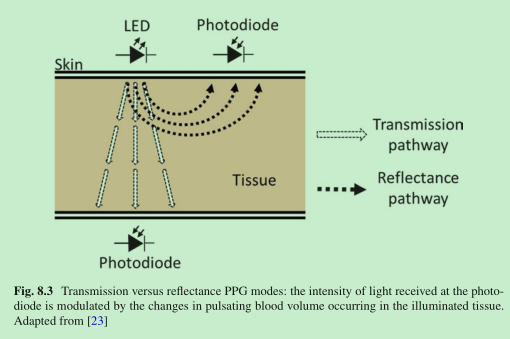
\includegraphics[width=.7\linewidth]{ch2/led}
    \caption{\label{fig:led}PPG检测的两种方式}
\end{figure}

当心脏收缩时外周血容量最多,光吸收量也最大,故检测到的光强度最小;而在心脏舒张时则恰恰相反,外周血容最小,光的吸收量最小,检测到的光强度最大\cite{lhc,cwl}。
由于人体指端区域毛细血管组织发达等优点,因此在光电容积脉搏波的临床中成为了检测位置的首选。\autoref{fig:ppgab}展示了人体指端各组织对光的吸收情况。
\begin{figure}[htb]
    \centering
    \includegraphics[width=.7\linewidth]{ch2/ppgab}
    \caption{\label{fig:ppgab}PPG信号的光吸收示意图}
\end{figure}

具体而言,物理光学中,将光通过某种透明介质后被吸收的比例定义为光的吸收度$A$,即:
\begin{equation}
    \label{equ:LBL}
    A=\lg\frac{I_{0}}{I_{T}}
\end{equation}

其中,$I_{0}$与$I_{T}$分别是入射光强度与透射光强度。而朗伯-比尔定律(Lambert-Beer's law)指出,光的吸收度与入射光的强度无关,在光程上每等厚层介质吸收相同比例值的光,即:
\begin{equation}
    \label{equ:LBL2}
    A=C \cdot \varepsilon \cdot V
\end{equation}

其中,$V$是透明介质的体积,$C$是透明介质的浓度,$\varepsilon$则是吸收系数,一般与透明介质的性质、入射光波长及温度等因素相关。

在透射式的光电检测中考虑到人体指端各组织对入射光的均有吸收,若忽略由于散射、反射等因素造成的衰减,以波长为$\lambda$的单色光垂直照射指端,则最终指端透射光强度为\cite{4122392}:
\begin{equation}
    \label{equ:AF1}
    I=I_{0}e^{-C_{t}\varepsilon _{t}V_{t}}e^{-C_{v}\varepsilon _{v}V_{v}} e^{-C_{a}\varepsilon _{a}V_{a}} 
\end{equation}

其中,下标$t$、$v$、$a$分别代表皮肤肌肉组织、静脉血液、动脉血液等成分。学者们已经证实皮肤肌肉组织、静脉血液等组织对光的吸收是恒定不变的\cite{1980Spectrophotometric,4122392}。
因此,可对\autoref{equ:AF1}进行精简,以表示通过动脉血液的透光强度\cite{PPGYY}:
\begin{equation}
    \label{equ:AF2}
    I=I_{0}e^{-C_{a}\varepsilon _{a}V_{a}} 
\end{equation}

当动脉血液的容积因心脏搏动而发生极小的变化$\Delta V_{a}$时,透光强度也将随之变动,将其记为$\Delta I$,则\autoref{equ:AF2}可改写为:
\begin{equation}
    \label{equ:AF3}
    I+\Delta I=I_{0}e^{-C_{a}\varepsilon _{a}(V_{a}+\Delta V_{a})} 
\end{equation}

将\autoref{equ:AF2}与\autoref{equ:AF3}相除,可得:
\begin{equation}
    \label{equ:AF4}
    \frac{I+\Delta I}{I}=\frac{I_{0}e^{-C_{a}\varepsilon _{a}(V_{a}+\Delta V_{a})}}{I_{0}e^{-C_{a}\varepsilon _{a}V_{a}}}=e^{-C_{a}\varepsilon _{a}\Delta V_{a}} 
\end{equation}

进一步,对\autoref{equ:AF4}两边同时取对数,并根据数学近似关系,若$x\rightarrow 0$,则$\ln(1+x)\approx x$,可得:
\begin{equation}
    \label{equ:AF5}
    \frac{\Delta I}{I}=-C_{a}\varepsilon _{a}\Delta V_{a}
\end{equation}

将\autoref{equ:AF2}代入\autoref{equ:AF5},稍作整理可得:
\begin{equation}
    \label{equ:AF6}
    \frac{\Delta V_{a}}{V_{a}}=\frac{1}{\ln(I/I_{0})}\frac{\Delta I}{I}
\end{equation}

即与个体相关性强的动脉血总的光吸收系数$\varepsilon _{a}$、动脉血浓度$C_{a}$等变量最终均与指端血液容积变化率无关,而后者与该容积透射的光强变化率$\Delta I/I$成正比例关系
\cite{1980Spectrophotometric,4122392,PPGYY}。PPG信号检测正是依此原理,通过光电转换
硬件电路检测光信号并从光强变化率中获取指端血液容积变化率的信息。
\section{小结}

\chapter{光电容积脉搏波数据源}
\section{引言}
\section{数据来源}
\section{人口统计学特征}
\section{采集设备}
\section{采集流程}
\section{脉搏波数据导出}
\section{小结}


\chapter{脉搏波特征点检测算法}

\chapter{及特征参数集的构建}
\section{引言}
\section{信号预处理}
\section{脉搏波波形检测及纠错}
\section{时域特征参数设计与特征集构建}
\subsection{角度、幅值、长度等}
\section{小结}

\chapter{基于数据特征集的模型构建}
\section{引言}

\section{数据来源}
\section{构建方法分析}
\section{模型构建}
\section{小结}

\chapter{模型评估}
\section{引言}
\section{评估方式与标准}
\section{具体模型表现对比}
\section{小结}

\chapter{低耦合、高拓展的软件综合分析系统的设计与实现}
\section{背景分析}
* 子痫前期检测的特定场景:孕妇、高龄、周期长、时间

* 实验室已有前期硬件研究基础,家俊研究基础

\section{需求分析:模块化、低耦合、高拓展}
* 多场景

* 特征计算拓展

* 数据管理

* 模型识别判断

\section{整体设计框图展示}

\section{各模块具体设计}
* 硬件采集支持

* 对数据源的拓展——多种数据格式均可兼容

* 对数据预处理的拓展——波形定位算法可拓展、纠错算法可拓展

* 对数据类型的拓展——目前只涉及脉搏波,但可方便拓展ECG等信号

* 对特征集构建拓展——方便随时研发新的特征参数进入特征集

\section{实现展示与测试}
界面
输入输出
\section{小结}

\chapter{总结与展望}
\section{研究工作总结}
\section{主要创新点}
* 提出了多种新型脉搏波特征参数,从时域形态特征方面构建了一般通用的脉搏波特征集

* 从特征集中筛选出对子痫前期具有识别能力的有效特征集合,并基于有效特征集合通过机器学习方法构建了子痫前期综合预测模型

* 设计并实现了一种低耦合、高拓展的方便类似研究工作开展的软件综合分析系统

\section{下一阶段工作展望}


% \begin{algorithm}

% \end{algorithm}